% Gorges (2021), "Of housewives and feminists", as a Lecture 3 game-theory case (detailed version).
% Compile: pdflatex housewives-game.tex (twice). Check: pdffonts (all Type 1, uni = yes).
% Every number is asserted by housewives-check.py in this folder. Page numbers "p. N" are the
% article's own pages 1-17 (Labour Economics 72, 102044).
\documentclass[11pt,a4paper]{article}
\usepackage[utf8]{inputenc}
\usepackage[T1]{fontenc}
\usepackage{lmodern}   % Type 1 vector fonts (replaces PK bitmaps)
\usepackage{cmap}      % ToUnicode CMap -> copyable text and accents
\usepackage[english]{babel}
\usepackage{amsmath,amssymb,amsthm,mathtools}
\usepackage{textcomp}
\usepackage[a4paper,margin=2.4cm]{geometry}
\usepackage{microtype}
\usepackage{booktabs,array,tabularx}
\usepackage{enumitem}
\usepackage{xcolor}
\usepackage{tikz}
\usepackage[most]{tcolorbox}
\usepackage{fancyhdr}
\usepackage{caption}
\usepackage[hidelinks]{hyperref}

\setlist{topsep=3pt,itemsep=2pt}
\setlength{\parindent}{0pt}
\setlength{\parskip}{5pt}
\renewcommand{\arraystretch}{1.2}
\allowdisplaybreaks
\captionsetup{font=small,labelfont=bf}

\pagestyle{fancy}\fancyhf{}
\lhead{\footnotesize Economics of Organizations and Incentives --- MPE Insper}
\rhead{\footnotesize Case: Of housewives and feminists as a game}
\cfoot{\footnotesize\thepage}
\renewcommand{\headrulewidth}{0.3pt}
\setlength{\headheight}{14pt}

\definecolor{ans}{RGB}{20,110,70}
\definecolor{src}{RGB}{30,80,150}
\definecolor{warn}{RGB}{190,90,20}
\newcommand{\answer}[1]{\begin{tcolorbox}[colback=ans!5,colframe=ans,boxrule=0.6pt,
  left=5pt,right=5pt,top=3pt,bottom=3pt]#1\end{tcolorbox}}
\newcommand{\ours}{\textcolor{warn}{\textbf{[Our analysis]}}}
\newcommand{\C}{\mathrm{C}}
\newcommand{\Fm}{\mathrm{F}}
\newcommand{\ECU}{\,\mathrm{ECU}}

\title{\textbf{Of Housewives and Feminists as a Game}\\[4pt]
  \large Battle of the sexes, mixed equilibrium, focal points and dynamics\\[2pt]
  \normalsize Case write-up for Lecture 3 --- Economics of Organizations and Incentives (MPE Insper)}
\date{November 2026}

\begin{document}
\maketitle
\thispagestyle{empty}

\begin{tcolorbox}[colback=src!4,colframe=src,boxrule=0.5pt,title={The case and how to read this write-up}]
\textbf{Paper.} Luise G\"orges (2021), ``Of housewives and feminists: Gender norms and
intra-household division of labour'', \emph{Labour Economics} 72, 102044. Page references
``p.~N'' are the article's pages 1--17; ``Table'' and ``fn.'' are the paper's own. The PDF is in
\texttt{Cases/Housewive and feminists/}.

\textbf{Lecture 3 link.} A one-shot battle of the sexes (BoS) solved in pure and mixed strategies
by the principle of indifference (Tadelis 2013, Ch.~6), then the sequential BoS solved by backward
induction and subgame perfection (Tadelis 2013, Ch.~7--8). Notation follows the slides: $p$ and $q$
are probabilities of the first action, $u_i$ expected payoffs.

\textbf{Labels.} Everything not stated in the paper is tagged \ours{} in the text. In particular the
independence computation of \S5, the own-payoff puzzle (\S6), the signal value (\S7), the
Fehr--Schmidt derivation (\S9) and the Lecture 5 preview (\S8.5) are ours. Amounts are in ECU
(1 ECU = 1 euro cent, p.~3). Every number is asserted by \texttt{housewives-check.py}.
\end{tcolorbox}

%--------------------------------------------------------------------------------------------
\section{The research question, the design and why a one-shot BoS}

\textbf{Question.} Do salient gender norms push couples toward a male-favouring division of
labour even when productivities, preferences and payoffs are held fixed? G\"orges frames
household specialisation as a coordination problem and asks whether the label ``Career/Family''
acts as a focal point (abstract, p.~1; p.~2).

\textbf{Design} (pp.~2--4).
\begin{itemize}
  \item \textbf{Subjects.} 192 subjects, real heterosexual couples, recruited from the Hamburg
    student pool; sessions in 2016 and 2017 (pp.~2, 4). Four sessions (80 participants) in
    \emph{Norm}, five (112) in \emph{Neutral} (p.~4).
  \item \textbf{Treatment.} Between subjects: the two actions are labelled \emph{Career} and
    \emph{Family} (Norm) or \emph{A} and \emph{B} (Neutral). The payoffs are identical (p.~3).
  \item \textbf{Pairing.} Within subjects: each subject plays once with the real partner and once
    with a randomly matched stranger of the same sex as the partner, order randomised (p.~4).
  \item \textbf{No communication.} Partners sit in closed booths and hand over their phones
    (fn.~11, p.~3; p.~4). Choices are revealed to the partner only ex post, after both rounds
    (fn.~14, p.~4; ``common knowledge that choices will be revealed ex-post'', p.~10).
\end{itemize}

\textbf{Why a one-shot BoS.} The paper calls the one-shot simultaneous game without communication
``a gross simplification'' but a deliberate one (p.~3): it creates the same non-cooperative
environment for all couples, so that Norm and Neutral and partner and stranger are comparable
(p.~4). Two further arguments (p.~4): (a) bargaining within the family may be non-cooperative, at
least at the threat point; (b) the ``first shot'' predicts later shots, because specialisation
feeds back into relative productivities (fn.~12, discussed in \S8.4). The structure also matches
the Lecture 3 BoS: two pure equilibria that each player ranks differently, plus a mixed one.

%--------------------------------------------------------------------------------------------
\section{The game}

\begin{itemize}
  \item \textbf{Players.} A woman $W$ and a man $M$ (the paper's Player 1 and Player 2).
  \item \textbf{Actions.} Each chooses $\C$ (Career, or $A$) or $\Fm$ (Family, or $B$).
  \item \textbf{Timing and information.} Simultaneous, one shot. Neither observes the other's
    action before moving. Payoffs and the rules are common knowledge (instructions, p.~4).
  \item \textbf{Payoffs} (Table 1, p.~3, with $\alpha=200$, $\beta=100$, $\alpha>\beta>0$): the
    player who chooses Career against a Family partner gets $\alpha$, the Family player gets
    $\beta$, and mis-coordination ($\C\C$ or $\Fm\Fm$) pays $0$ to both.
\end{itemize}

\begin{center}
\begin{tabular}{cc|cc}
 & & \multicolumn{2}{c}{\textbf{Man}}\\
 & & $\C$ & $\Fm$ \\ \hline
\textbf{Woman} & $\C$ & $0,\ 0$ & $\mathbf{200},\ \mathbf{100}$ \\
 & $\Fm$ & $\mathbf{100},\ \mathbf{200}$ & $0,\ 0$ \\
\end{tabular}
\end{center}
(Payoffs listed as woman, man. Bold: the two pure Nash equilibria.)

Features that the paper designs in (p.~3): payoffs favour the Career player, they are
\emph{symmetric across the two equilibria} (total 300 either way; same for both sexes), and they
do not change across treatments. The total is highest when one partner specialises in each task,
which reflects gains from specialisation in the production function (fn.~7), not comparative
advantage. The asymmetry $\alpha>\beta$ can reflect control over earnings, a better outside
option after divorce, or a taste for Career (p.~3).

%--------------------------------------------------------------------------------------------
\section{Equilibria of the one-shot BoS}

\subsection{Pure strategies}
Check each cell. At $(\C,\Fm)$ the woman gets $200$ and would get $0$ by moving to $\Fm$; the man
gets $100$ and would get $0$ by moving to $\C$. So $(\C,\Fm)$ is a Nash equilibrium (NE), and by
symmetry so is $(\Fm,\C)$. At $(\C,\C)$ each gets $0$ and would get $100$ by switching to $\Fm$;
likewise at $(\Fm,\Fm)$ each would gain $200$ by switching to $\C$. The paper's words for the two
NE (p.~3): $(\C,\Fm)$ is \emph{Progressive} (female-favouring), $(\Fm,\C)$ is \emph{Traditional}
(male-favouring). Each player prefers the equilibrium in which she or he is the Career player.

\subsection{The mixed equilibrium by the principle of indifference}
Let $p=\Pr(W\text{ plays }\C)$ and $q=\Pr(M\text{ plays }\C)$. Against a man who plays $\C$ with
probability $q$ the woman's expected payoffs are
\[
u_W(\C,q)=(1-q)\cdot 200+q\cdot 0=200(1-q),\qquad
u_W(\Fm,q)=q\cdot 100+(1-q)\cdot 0=100\,q .
\]
She prefers $\C$ iff $200(1-q)>100q\iff 200>300q\iff q<\tfrac23$; she prefers $\Fm$ iff
$q>\tfrac23$; she is indifferent iff $q=\tfrac{\alpha}{\alpha+\beta}=\tfrac23$. The principle of
indifference says that a player mixes only if every action in her support gives the same
expected payoff, so the \emph{man's} mix is pinned down by the \emph{woman's} payoffs:
$q^*=\tfrac23$. By the symmetric argument for the man,
\[
u_M(\C,p)=200(1-p),\quad u_M(\Fm,p)=100\,p\ \Rightarrow\ p^*=\tfrac23 .
\]

\answer{\textbf{Mixed NE.} Each player chooses Career with probability $\tfrac{\alpha}{\alpha+\beta}=\tfrac23$
and Family with $\tfrac13$ (paper, p.~3). Expected payoff
$u_W=u_M=200\left(1-\tfrac23\right)=\tfrac{\alpha\beta}{\alpha+\beta}=\tfrac{200}{3}\approx66.7$ ECU,
``nearly 67 ECU'' (p.~3), which is only $\tfrac23$ of the $\beta=100$ a player gets in her worse pure
equilibrium.}

\textbf{Best-response diagram.} The woman's best response to $q$ is $p=1$ for $q<\tfrac23$, any $p$ at
$q=\tfrac23$ and $p=0$ for $q>\tfrac23$; the man's is $q=1$ for $p<\tfrac23$, any $q$ at
$p=\tfrac23$ and $q=0$ for $p>\tfrac23$. Equilibria are the intersections.

\begin{center}
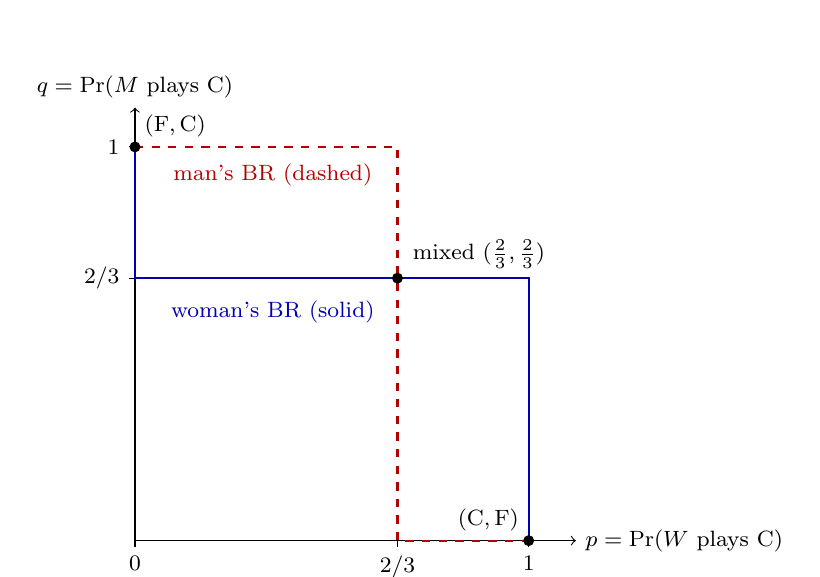
\begin{tikzpicture}[scale=5,every node/.style={font=\footnotesize}]
  \draw[->] (0,0) -- (1.12,0) node[right]{$p=\Pr(W\text{ plays }\C)$};
  \draw[->] (0,0) -- (0,1.1) node[above]{$q=\Pr(M\text{ plays }\C)$};
  \foreach \x/\l in {0/0,0.6667/{2/3},1/1} { \draw (\x,0.015) -- (\x,-0.015) node[below]{$\l$}; }
  \foreach \y/\l in {0.6667/{2/3},1/1} { \draw (0.015,\y) -- (-0.015,\y) node[left]{$\l$}; }
  \draw[thick,blue!70!black] (1,0) -- (1,0.6667) -- (0,0.6667) -- (0,1);
  \draw[thick,red!70!black,dashed] (0,1) -- (0.6667,1) -- (0.6667,0) -- (1,0);
  \node[circle,fill,inner sep=1.4pt] at (1,0) {};
  \node[circle,fill,inner sep=1.4pt] at (0,1) {};
  \node[circle,fill,inner sep=1.4pt] at (0.6667,0.6667) {};
  \node[above left] at (1,0) {$(\C,\Fm)$};
  \node[above right] at (0.0,1.0) {$(\Fm,\C)$};
  \node[above right,xshift=2pt] at (0.6667,0.6667) {mixed $(\tfrac23,\tfrac23)$};
  \node[blue!70!black] at (0.35,0.58) {woman's BR (solid)};
  \node[red!70!black] at (0.35,0.93) {man's BR (dashed)};
\end{tikzpicture}

{\footnotesize Three intersections: two pure equilibria at the corners and the mixed one at $(\tfrac23,\tfrac23)$.}
\end{center}

\subsection{What the mixed equilibrium implies for outcomes}
If both mix independently, the four cells have probabilities
\[
\Pr(\C,\Fm)=\tfrac23\cdot\tfrac13=\tfrac29,\quad
\Pr(\Fm,\C)=\tfrac13\cdot\tfrac23=\tfrac29,\quad
\Pr(\C,\C)=\tfrac23\cdot\tfrac23=\tfrac49,\quad
\Pr(\Fm,\Fm)=\tfrac13\cdot\tfrac13=\tfrac19 .
\]
So Progressive $\tfrac29$, Traditional $\tfrac29$, both-Career $\tfrac49$, both-Family $\tfrac19$ (they
sum to $1$). Coordination (Progressive or Traditional) happens with probability
$\tfrac29+\tfrac29=\tfrac49\approx44.4\%$, ``just below 45\%'' (p.~3); this is the dotted line in the
paper's Fig.~2. Check of the payoff: the woman gets $200$ in the Progressive cell and $100$ in the Traditional one,
so $\tfrac29\cdot200+\tfrac29\cdot100=\tfrac{600}{9}=\tfrac{200}{3}$, the same as above (and by
symmetry for the man).

\subsection{Efficiency comparison}
In either pure NE the pair earns $200+100=300$. In the mixed NE it earns
$2\times\tfrac{200}{3}=\tfrac{400}{3}\approx133.3$, less than half. The mixed equilibrium is
symmetric and ex ante equal, but wastes more than half of the surplus on mis-coordination
(probability $\tfrac59$). The pure equilibria are efficient but unequal ($200$ against $100$).
\emph{This is the efficiency--equality trade-off} that the paper's conclusion stresses (p.~11).

%--------------------------------------------------------------------------------------------
\section{Focal points: what the Norm label should do}

The BoS has three equilibria and the theory does not say which is played. Schelling (1960): in a
coordination problem a salient feature, unrelated to the payoffs, can lead players to expect the
same equilibrium. The paper's hypothesis (p.~3): when actions are labelled Family and Career,
``the `traditional', male-favouring, equilibrium would be reached more often, thus improving
efficiency at the cost of increased inequality to the disadvantage of women''.

\textbf{Mechanism in game-theoretic terms.} A focal point does not alter payoffs. It changes
\emph{beliefs}: if the woman expects the man to play $\C$ with probability above $\tfrac23$, her best
response is $\Fm$ (from the indifference condition above); if the man expects $\Fm$ from the woman
with high enough probability, $\C$ is his best response. Beliefs that point to the Traditional cell
are self-fulfilling, hence an equilibrium. Neutral labels ($A$/$B$) give no such pointer, so the
prediction there is the symmetric mixed benchmark (or a weak pull of the first-listed action).

\textbf{Predictions for Norm versus Neutral} (p.~3, and the \emph{a priori} expectation on p.~7):
(i) Traditional rises and Progressive falls; (ii) coordination rises; (iii) women choose Career less
and men more. \textbf{Welfare.} Total payoff rises toward $300$ per couple, but all of the gain in
\emph{inequality} goes to the man: the Traditional cell pays him $200$ and her $100$. The Norm
label moves society along the efficiency--equality trade-off, with no change in fundamentals.

%--------------------------------------------------------------------------------------------
\section{Confronting theory with the data}

\subsection{What the paper reports}
\begin{itemize}
  \item \textbf{Career rates} (Table 4, col.~1, p.~8; text p.~7). Men, Neutral: $0.536$ (intercept);
    women, Neutral: $0.536+0.027=0.563$; men, Norm: $0.536+0.089=0.625$; women, Norm:
    $0.536+0.089+0.027-0.402=0.250$. $N=384$ (192 subjects $\times$ 2 pairings).
    Women's rate falls by $0.313$, ``by more than half'' (p.~11); men's rise by $0.089$, not significant.
  \item \textbf{Outcomes} (Table 3, col.~2, p.~6; text p.~7): moving from Neutral to Norm changes the
    probability of the Progressive outcome by $-0.171$, of the Traditional by $+0.255$, of
    non-coordination by $-0.085$ (not significant, $p=0.29$).
  \item \textbf{Earnings} (Table C1, p.~15): Norm men $112.50$, women $75.00$; Neutral men
    $80.36$, women $83.04$. Women in Norm earn $75.00/112.50=\tfrac23$, ``67\% of men'' (p.~7).
\end{itemize}

\subsection{Best responses against the real rates}
\ours{} Take the observed rates as the opponent's mix.
\textbf{Woman in Norm} facing men who choose $\C$ with probability $q=0.625$:
\[
u_W(\C)=(1-0.625)\cdot200=75,\qquad u_W(\Fm)=0.625\cdot100=62.5 .
\]
Career was her best response, though only just ($0.625<\tfrac23$; the gap to the indifference point
is $\tfrac1{24}$). Yet only $25\%$ of women chose it. \textbf{Man in Norm} facing women's $p=0.25$:
$u_M(\C)=0.75\cdot200=150$, $u_M(\Fm)=0.25\cdot100=25$; Career is strongly best, yet $62.5\%$ chose
it. In Neutral, against men's $0.536$ the woman gets $92.8$ from $\C$ and $53.6$ from $\Fm$; the
man against women's $0.563$ gets $87.4$ and $56.3$: Career is the best response in both
frames.

\subsection{Beliefs explain women, not men}
Best responses are against \emph{beliefs}. The paper elicits them (\S5.1, pp.~8--9): women's
predicted male Career rates are ``substantially higher than the true rates'' (fn.~27, p.~9), while
``men greatly overestimate women's rate of choosing Career in the Norm group'' (p.~9). A woman who
believes $q>\tfrac23$ has $\Fm$ as best response, which matches women's behaviour. The paper
concludes that beliefs ``seem to explain Career choices for women'' but not men's differential
response to partner versus stranger (p.~9). Overshooting beliefs about men's Career-playing are
what a Schelling focal point does: the Norm label makes ``he will take Career'' the expectation.

\subsection{Independence benchmark (ours, not the paper's)}
\ours{} \emph{This computation is ours: the paper does not report it.} If the woman plays $\C$ with
the observed probability $p$ and the man with $q$, independently, the outcome rates are
$\Pr(\text{Prog})=p(1-q)$ and $\Pr(\text{Trad})=(1-p)q$.

\begin{center}
\begin{tabular}{lcccc}
\toprule
 & $p$ (women) & $q$ (men) & Progressive & Traditional \\
\midrule
Neutral & $0.563$ & $0.536$ & $0.563\times0.464=0.261$ & $0.437\times0.536=0.234$ \\
Norm    & $0.250$ & $0.625$ & $0.250\times0.375=0.094$ & $0.750\times0.625=0.469$ \\
\bottomrule
\end{tabular}
\end{center}
Coordination: Neutral $0.261+0.234=0.495$, Norm $0.094+0.469=0.5625$. Both exceed the
mixed-equilibrium $\tfrac49=0.444$, and Norm exceeds Neutral, as a focal point predicts. Expected
earnings in Norm under independence (man earns $200$ in the Traditional cell and $100$ in the
Progressive): men $200\times0.469+100\times0.094=103.1$, women $100\times0.469+200\times0.094=65.6$.
In Neutral: men $73.0$, women $75.7$.

\textbf{Observed versus independence.} Table C1 gives $112.50$ and $75.00$ in Norm and $80.36$ and
$83.04$ in Neutral. All four are above the independence figures: by $9.4$ for both sexes in Norm
($112.50-103.1$, $75.00-65.6$) and by about $7.4$ in Neutral. Pairs coordinate more than
independent play implies. A second \ours{} check:
a coordinated pair pays $300$ in total and a mis-coordinated pair $0$, so total earnings$/300$ is the
implied coordination rate: Norm $(112.50+75.00)/300=0.625$, Neutral $(80.36+83.04)/300=0.545$.
The gap, $0.080$, is close to Table 3's $-0.085$ on non-coordination. The total payoff per couple
rises from $163.4$ to $187.5$ ($+24.1$), while the male--female gap goes from $-2.68$
(women ahead) to $+37.5$. Men gain $32.14$ ECU and women lose $8.04$.

%--------------------------------------------------------------------------------------------
\section{The own-payoff puzzle (our analysis)}

\ours{} A tempting reading of the Norm label is as a \emph{payoff} effect: women get an identity
utility $n>0$ from choosing Family (a ``housewife'' norm), added whatever the partner does.
Does this fit the data? Redo the indifference condition:
\[
u_W(\C,q)=200(1-q),\qquad u_W(\Fm,q)=100\,q+n .
\]
The woman is indifferent iff $200-200q=100q+n$, so
\[
q^*(n)=\frac{200-n}{300}.
\]
The man's payoffs are unchanged, so his indifference still gives $p^*=\tfrac23$. In the
\emph{mixed} equilibrium therefore the identity utility changes the \emph{man's} mix, not the woman's.
For $n=0,50,100,150$ the man's $\Pr(\C)$ is $\tfrac23,\tfrac12,\tfrac13,\tfrac16$. (For $n\ge200$,
Family is dominant for her and $(\Fm,\C)$ is the unique NE.)

\textbf{Reading.} The principle of indifference makes each player's mix depend on the
\emph{other} player's payoffs. A payoff shift for women inside the mixed equilibrium would move
men's behaviour and leave women's at $\tfrac23$. The data show the opposite: women fall from
$0.563$ to $0.250$ and men are about flat ($0.536\to0.625$, not significant). This points to
\textbf{equilibrium selection} (a focal point and beliefs, \S4) rather than a payoff shift in a
mixed equilibrium. A caveat: if play was in a pure-strategy equilibrium with heterogeneity in $n$
across women, a payoff story could also fit; we cannot separate them with this design, and the
paper's own design (payoffs identical across treatments, p.~3) is meant to rule out payoff
differences.

%--------------------------------------------------------------------------------------------
\section{Men ``acting feminist'' (\S5.2): a preview of signalling}

Men react little to the Norm label with their real partner but more with strangers (p.~7). The
paper's explanation (\S5.2, p.~10): choices are revealed ex post to the partner, and men in
non-committed relationships may want to signal progressive attitudes to a potential long-term
partner. Their Career rates (p.~10): with the real partner, $33\%$ in Norm versus $54\%$ in
Neutral ($p=0.07$); with strangers, $78\%$ in Norm versus $48\%$ ($p=0.01$). The gap is $21$
percentage points with the partner and about $45$ points between partner and stranger in Norm.
The subgroup of committed couples is small ($n=30$ Neutral, $22$ Norm, p.~10).

\ours{} \textbf{How big must the signal be?} Take a man in Norm who believes his partner plays $\C$
with probability $0.33$: in Norm, $33\%$ of men predict that their partner chose Career, against
$66\%$ for their stranger (\S5.1, p.~9, $p=0.01$). Then
\[
u_M(\C)=0.67\cdot200=134,\qquad u_M(\Fm)=0.33\cdot100=33 .
\]
Choosing Family costs him $134-33=101$ ECU (\texteuro{}1.01) in expectation, so
the benefit of signalling must exceed $101$ ECU for $\Fm$ to be rational. Against the women's actual
$0.25$ the cost would be $150-25=125$. The paper itself notes that Family in a low-stakes lab game
is ``a particularly easy and cheap way'' to signal (fn.~29, p.~10) and that whether women find it
credible is open. Beyond this number we stay qualitative: it is a preview of signalling games
(Lecture 8), where a costly action is chosen because of what it reveals about the sender's type
to an observer, and where the equilibrium depends on the observer's beliefs.

%--------------------------------------------------------------------------------------------
\section{Dynamics: the sequential BoS, commitment, path dependence}

\subsection{Sequential BoS and backward induction}
Suppose one partner moves first and the other observes the move (Lecture 3 slides: Alex reaches
the venue first and calls Chris; here: the partner who makes the first career commitment, the
first job offer or the first child decision). Let the woman move first.
After $\C$ the man chooses between $\C$ ($0$) and $\Fm$ ($100$): he plays $\Fm$. After $\Fm$ he chooses
between $\C$ ($200$) and $\Fm$ ($0$): he plays $\C$. Knowing this the woman compares $\C\to200$ with
$\Fm\to100$ and plays $\C$.

\begin{center}
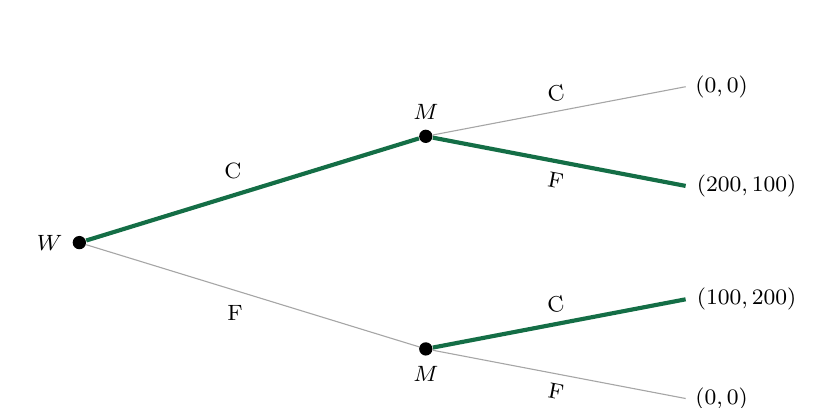
\begin{tikzpicture}[x=1.1cm,y=0.9cm,every node/.style={font=\footnotesize},
  dec/.style={circle,fill,inner sep=1.7pt},
  spe/.style={draw=ans,line width=1.5pt},e/.style={draw=gray!70}]
  \node[dec,label=left:$W$] (r) at (0,0) {};
  \node[dec,label=above:$M$] (a) at (4,1.5) {};
  \node[dec,label=below:$M$] (b) at (4,-1.5) {};
  \draw[spe] (r) -- node[above left]{$\C$} (a);
  \draw[e] (r) -- node[below left]{$\Fm$} (b);
  \draw[e] (a) -- node[above,sloped]{$\C$} (7,2.2) node[right]{$(0,0)$};
  \draw[spe] (a) -- node[below,sloped]{$\Fm$} (7,0.8) node[right]{$(200,100)$};
  \draw[spe] (b) -- node[above,sloped]{$\C$} (7,-0.8) node[right]{$(100,200)$};
  \draw[e] (b) -- node[below,sloped]{$\Fm$} (7,-2.2) node[right]{$(0,0)$};
\end{tikzpicture}

{\footnotesize Payoffs (woman, man). Thick green: the subgame-perfect equilibrium (SPE). The woman's
choice at the root is $\C$; the man plays $\Fm$ after $\C$ and $\C$ after $\Fm$.}
\end{center}

\answer{\textbf{SPE} (woman first): $W$ plays $\C$; $M$ plays $\Fm$ after $\C$ and $\C$ after $\Fm$. Payoffs
$(200,100)$. The first mover gets $200$, against $\tfrac{200}{3}\approx66.7$ in the simultaneous
mixed NE, a gain of $\tfrac{400}{3}\approx133.3$, and against $100$ if she were the second mover.}

\subsection{Nash equilibria that are not subgame perfect}
The man has four contingent plans (action after $\C$, action after $\Fm$) and the woman two
actions, so eight profiles. Checking best responses gives three pure NE:
$(\C;\ \Fm,\C)$ (the SPE), $(\C;\ \Fm,\Fm)$ (same outcome, an irrelevant off-path action) and
$(\Fm;\ \C,\C)$, with payoffs $(100,200)$. The last is built on the threat \emph{``I play Career
whatever you do''}: it deters the woman from playing $\C$, because then she would get $0$. But after
$\C$ the man would get $0$ from carrying it out and $100$ from $\Fm$, so the threat is not credible,
and the continuation after $\C$ is not a Nash equilibrium of that subgame. Subgame perfection removes it.

\subsection{Commitment and the value of moving first}
The sequential game turns the BoS into one where \emph{being first is worth $133$ ECU}. The
paper's setting is simultaneous, but real households have precisely this structure: whoever gets the
job offer, the promotion or the first child first creates facts the other must best-respond to.
Visible commitment beats talk (cheap talk is excluded by design, fn.~11).

\subsection{Path dependence (fn.~12, p.~4)}
The paper argues that today's specialisation changes tomorrow's payoffs: ``the equilibrium in which
spouses choose the same actions as in a past game now generates higher individual and total
payoffs than before, thus increasing the likelihood that spouses coordinate on it'' (fn.~12).
The first shot is therefore the most relevant (p.~4). In game terms, a stage-game equilibrium
becomes a state variable of the next stage game, so the initial selection (the focal point!) can be
locked in.

\subsection{Preview of Lecture 5 (our analysis)}
\ours{} In the repeated game the partners could \emph{alternate} the two pure equilibria,
$(\C,\Fm),(\Fm,\C),\dots$, giving each $\tfrac{200+100}{2}=150$ per period, against $\tfrac{200}{3}$
for repeating the mixed NE. A sequence of stage-game Nash equilibria is a subgame-perfect equilibrium
of a finitely repeated game (Lecture 5). Yet the paper's own argument (fn.~12) is that specialisation
feeds back into wages, so the symmetric alternation is costly to sustain: the Career spouse's
productivity advantage is exactly the state variable that breaks the symmetry of payoffs.

%--------------------------------------------------------------------------------------------
\section{Inequality aversion: when does coordination survive? (fn.~13)}

The paper notes that inequality aversion would have to be ``rather pronounced to alter the
pure-strategy equilibria (2 and 1 for advantageous and disadvantageous inequality aversion,
respectively, in a Fehr and Schmidt (1999) model)'' (fn.~13, p.~4). \ours{} \emph{Derivation.} With
Fehr--Schmidt utility
\[
U_i(x_i,x_j)=x_i-\alpha_{FS}\max\{x_j-x_i,0\}-\beta_{FS}\max\{x_i-x_j,0\},
\]
($\alpha_{FS}$ weighs disadvantageous inequality, $\beta_{FS}$ advantageous; subscript FS to avoid
clashing with the payoffs $\alpha,\beta$), consider $(\C,\Fm)$ with payoffs $(200,100)$.
\begin{itemize}
  \item The Career player is advantaged: $U=200-100\,\beta_{FS}$. By deviating to $\Fm$ she reaches
    $(\Fm,\Fm)$ with payoffs $(0,0)$, no inequality, $U=0$. She stays iff $200-100\beta_{FS}>0\iff
    \beta_{FS}<2$.
  \item The Family player is disadvantaged: $U=100-100\,\alpha_{FS}$. By deviating to $\C$ he reaches
    $(\C,\C)$ with $U=0$. He stays iff $100-100\alpha_{FS}>0\iff\alpha_{FS}<1$.
\end{itemize}
\answer{Coordination remains a (strict) Nash equilibrium iff $\beta_{FS}<2$ and $\alpha_{FS}<1$ (with
equality, weak). This matches the paper's ``2 and 1''. The paper's judgement (fn.~13) is that inequality aversion would have to be
rather pronounced to remove the pure equilibria, so it does not model it as a motive; beyond that
we do not use outside estimates of $\alpha_{FS},\beta_{FS}$.}

%--------------------------------------------------------------------------------------------
\section{Limits and critique}

\begin{itemize}
  \item \textbf{Lab, stakes.} Stakes are small and the paper says so (fn.~6, p.~3: behaviour in
    strategic games is ``largely invariant to stake size''). Session payouts averaged
    \texteuro{}27.43 (p.~4), and the game took 10 minutes in a 2.5 hour session.
  \item \textbf{Sample.} 192 students from the Hamburg lab, recruited in 2016--17 (p.~4);
    ``a small, highly selected sample'' (p.~11). Norm and Neutral are assigned by session, so
    the treatment varies at the session level (4 against 5 sessions, fn.~21). Participants differ in
    age ($25$ against $27$ years, p.~5).
  \item \textbf{One shot.} Real specialisation is repeated and has commitment and path
    dependence (\S8); the one-shot game isolates the first shot but not the dynamics.
  \item \textbf{Payoff structure.} Symmetric totals mean no efficiency reason to prefer either
    equilibrium. Real households have productivity and preference differences correlated with norms
    (p.~3).
  \item \textbf{Unobserved mechanism.} The signalling reading was not designed in (p.~10), the
    committed subgroup is small ($22$--$30$), and ``the puzzle of men's differential response'' is left unresolved by beliefs (p.~9).
  \item \textbf{Our modelling choices.} Independence of the two choices (\S5.4) is an assumption;
    pairs may share unobserved traits, and the repeated play over partner and stranger pairings is
    not independent either.
\end{itemize}

%--------------------------------------------------------------------------------------------
\section{Discussion questions}

\textbf{Q1. In Neutral the mixed NE predicts $44.4\%$ coordination. Why might observed coordination
be higher?}
\answer{The implied rate from Table C1 is $0.545$, and from independent play $0.495$. The mixed NE
assumes symmetric, independent randomisation; plausibly subjects use shared salience (the
order of the labels, a convention about who takes the larger payoff), which correlates choices.
That is a focal point acting even without an explicit label; the paper does not test it.}

\textbf{Q2. Is a focal point an equilibrium refinement?}
\answer{No. All three equilibria survive in the Norm game, as payoffs are unchanged. A focal point is
a selection device acting through beliefs: it makes one equilibrium the common expectation and,
once believed, it is self-confirming. It is not derived from the payoffs.}

\textbf{Q3. A woman in Norm faces men who play Career $62.5\%$ of the time. What does she earn from
Career and from Family, and why did $75\%$ of women choose Family?}
\answer{Career pays $75$ and Family $62.5$. Against the true rate, Career is the best response. A woman
who believes men choose Career with probability above $\tfrac23$ prefers Family. Women's beliefs
overshoot the true rates (fn.~27), so Family was a best response to their beliefs. The price of the
overshoot, under independence, is $75-65.6=9.4$ ECU per game in expectation (ours).}

\textbf{Q4. Could the Norm effect be a change in women's payoffs?}
\answer{If women get identity utility $n$ from Family, the mixed NE moves the \emph{men's} mix to
$\tfrac{200-n}{300}$ and leaves the women's at $\tfrac23$. The data move the women. A payoff shift in
a mixed NE does not predict this, so equilibrium selection (beliefs) is the better account (ours).}

\textbf{Q5. Why would a non-committed man choose Family in front of his partner?}
\answer{With the belief $0.33$ his expected payoff loss is $101$ ECU ($\approx$ \texteuro{}1). It is rational only
if the signalling gain from showing progressive attitudes exceeds $101$ ECU. The paper stays
cautious (fn.~29; it was not designed to test the hypothesis) and Lecture 8 gives the tools: a
signal is credible if its cost differs across types.}

\textbf{Q6. Does the Norm label improve welfare?}
\answer{Total earnings per couple rise from $163.4$ to $187.5$ ECU, and the Traditional equilibrium is
efficient, but women lose $8.04$ and men gain $32.14$. Whether this is an improvement depends on the
weight on equality; the paper does not choose (p.~11). With sequential moves (first mover gets
$200$) or alternation ($150$ each) the same efficiency is attainable with less inequality ---
but only if the households can commit or take turns, which fn.~12 suggests is hard.}

\end{document}
